% !TEX TS-program = pdflatex
% !TEX encoding = UTF-8 Unicode

% This is a simple template for a LaTeX document using the "article" class.
% See "book", "report", "letter" for other types of document.

\documentclass[11pt]{article} % use larger type; default would be 10pt

\usepackage[utf8]{inputenc} % set input encoding (not needed with XeLaTeX)

%%% Examples of Article customizations
% These packages are optional, depending whether you want the features they provide.
% See the LaTeX Companion or other references for full information.

%%% PAGE DIMENSIONS
\usepackage{geometry} % to change the page dimensions
\geometry{a4paper} % or letterpaper (US) or a5paper or....
\geometry{margin=1in} % for example, change the margins to 2 inches all round
% \geometry{landscape} % set up the page for landscape
%   read geometry.pdf for detailed page layout information

\usepackage{graphicx} % support the \includegraphics command and options

% \usepackage[parfill]{parskip} % Activate to begin paragraphs with an empty line rather than an indent

%%% PACKAGES
\usepackage{booktabs} % for much better looking tables
\usepackage{array} % for better arrays (eg matrices) in maths
\usepackage{paralist} % very flexible & customisable lists (eg. enumerate/itemize, etc.)
\usepackage{verbatim} % adds environment for commenting out blocks of text & for better verbatim
\usepackage{subfig} % make it possible to include more than one captioned figure/table in a single float
\usepackage{amsmath}
\usepackage{bbm}
\usepackage{amssymb}
\usepackage{graphicx}
\usepackage{algorithm}
\usepackage{url}
\usepackage{cite}
\usepackage[noend]{algpseudocode}
% These packages are all incorporated in the memoir class to one degree or another...

%%% HEADERS & FOOTERS
\usepackage{fancyhdr} % This should be set AFTER setting up the page geometry
\pagestyle{fancy} % options: empty , plain , fancy
\renewcommand{\headrulewidth}{0pt} % customise the layout...
\lhead{}\chead{}\rhead{}
\lfoot{}\cfoot{\thepage}\rfoot{}

%%% SECTION TITLE APPEARANCE
\usepackage{sectsty}
\allsectionsfont{\sffamily\mdseries\upshape} % (See the fntguide.pdf for font help)
% (This matches ConTeXt defaults)

%%% ToC (table of contents) APPEARANCE
\usepackage[nottoc,notlof,notlot]{tocbibind} % Put the bibliography in the ToC
\usepackage[titles,subfigure]{tocloft} % Alter the style of the Table of Contents
\renewcommand{\cftsecfont}{\rmfamily\mdseries\upshape}
\renewcommand{\cftsecpagefont}{\rmfamily\mdseries\upshape} % No bold!

%%% >>>>>> SHORTCUTS>>>>>>
\DeclareMathOperator{\E}{E}
\DeclareMathOperator{\Var}{Var}
\DeclareMathOperator{\Cov}{Cov}
\DeclareMathOperator{\argmin}{argmin}
\DeclareMathOperator{\argmax}{argmax}
\newcommand{\pr}{^{(pr)}}

%%% END Article customizations

%%% The "real" document content comes below...

\title{Table parsing notes}
\author{Alex Ratner}
%\date{} % Activate to display a given date or no date (if empty),
         % otherwise the current date is printed 

\begin{document}
\maketitle

% - What does user provide?
%   - distant supervision?
%   - [Active Learning??] can we have some entropy metric to provide most diverse set of tables to label?
%   - features for tables?
% - Do we need hard constraints?  And do we need these in a setting w structure??

% --> define table complexity metric for error analysis!

% declarative language
% - in ddlog?  For table constraints?
% - PCFG system?  (is this necessary?)

\section{Motivating examples}

\subsection{SEC Filings}
\begin{figure}[h]
    \centering
    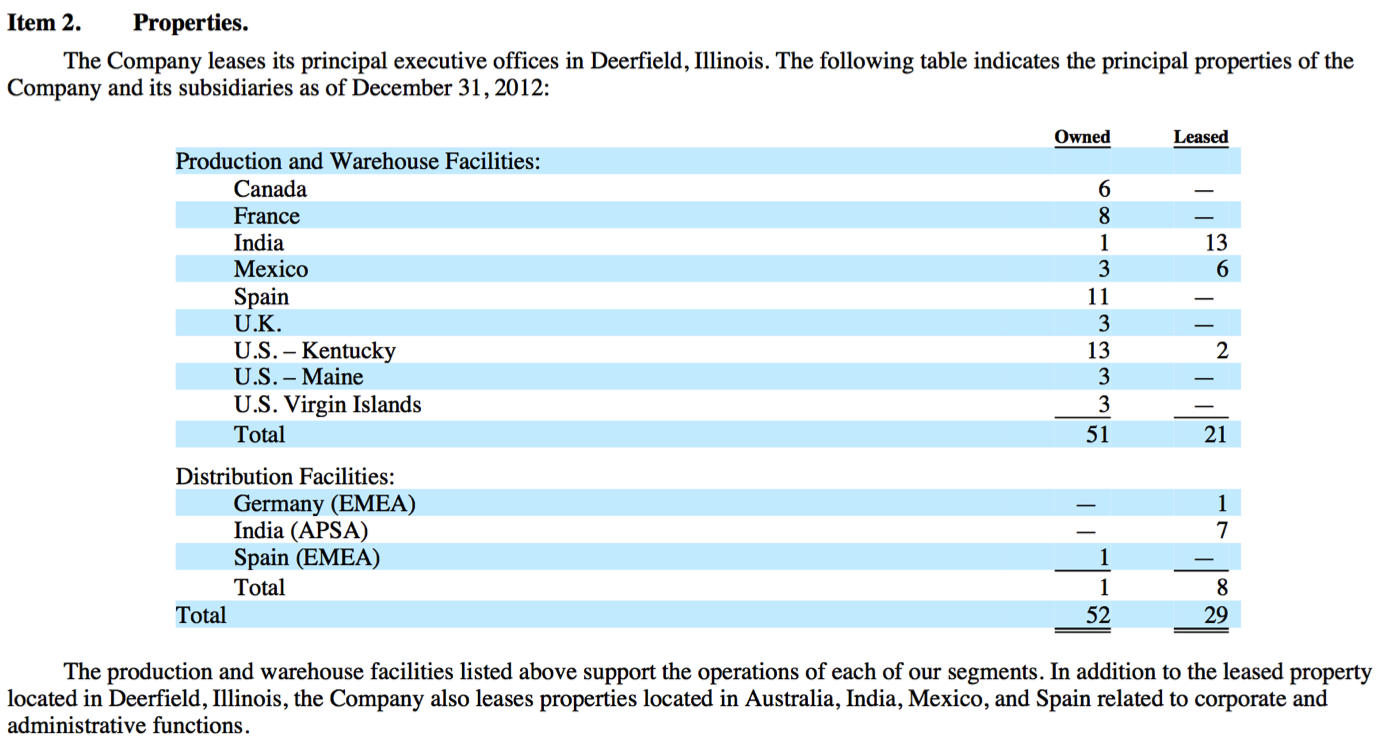
\includegraphics[width=1.0\textwidth]{sec_table_1.png}
    \caption{Property ownership overview table from Beam Inc's 10-K}
    \label{fig:sec_table_1}
\end{figure}

Suppose we wish to extract $(\text{Production facility location}, \text{Production facility quantity})$ tuples, for owned properties, from SEC filings.  Suppose that we define candidate entities for this tuple as any capitalized phrase and number respectively.  We would hope to ultimately extract e.g. $(\text{U.S.-Kentucky}, 13)$, but not $(\text{U.S.-Kentucky}, 2)$, $(\text{Germany (EMEA)}, \text{-})$, or $(\text{Total}, 51)$.

A single line / sentence, corresponding to our atomic processing unit, might look like:
\begin{verbatim}
<tr><td>\tU.S. - Kentucky</td><td>13</td><td>2</td></tr>
\end{verbatim} 
The crux of our task is then to enable the use of \textit{global} features i.e. feature function inputs from beyond this line, having to do with the overall structure of the table, such as:
\begin{verbatim}
<b><u>Owned</u></b>
Production and Warehouse Facilities:
<b>Item 2.\tProperties.
CATEGORY_HEADER=False
SUMMARY_LINE=False
\end{verbatim}
We see here that \textbf{parsing the table's structure} is a tertiary task to our secondary task of \textbf{extracting \textit{attributes}}- e.g. column labels, row labels, etc.- connected to candidate entities in our primary \textbf{relation extraction} task.

One hypothesis is that to accomplish this, a simple parsing of the table structure can be used- i.e. in contrast to something like a 2D PCFG like in \cite{Lee_2006}.  For example in \cite{McCallum_2003}, a CRF is used to label rows of ASCII text tables with certain table type labels (including 'not a table', crucial in their scenario).  Especially with data from a slightly more structured format, e.g. XML or HTML, where columns are more deterministicly resolved, these types of labels might be sufficient information for determining which attributes are related to a given entity / cell.

The rough idea would then be to do this table row categorization task \textbf{jointly} with our primary relation extraction task.

\subsection{Genomics / Scientific Literature}
\begin{figure}[h]
    \centering
    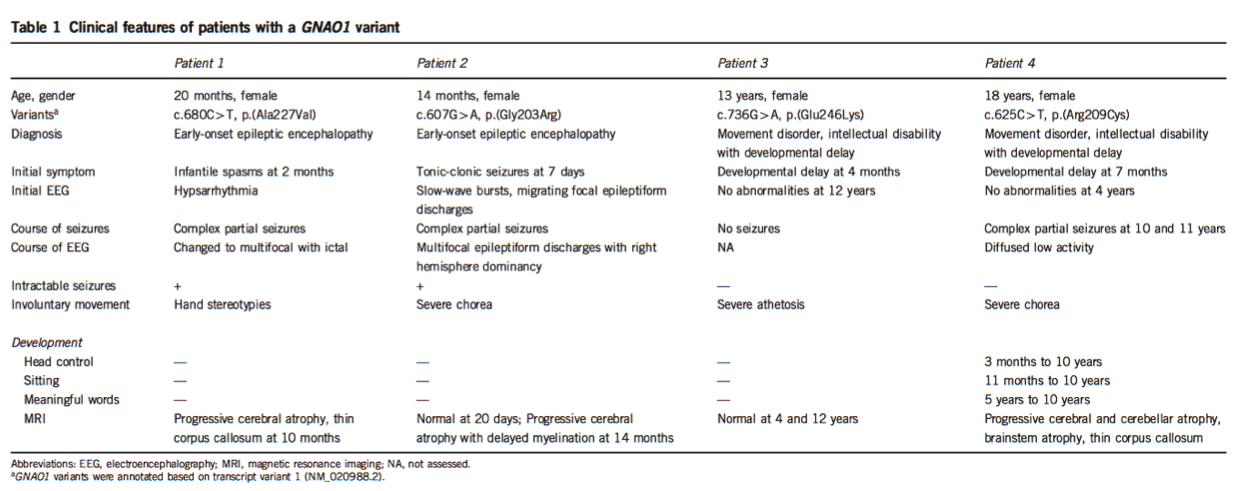
\includegraphics[width=1.0\textwidth]{genomics_table_1.png}
    \caption{A table in a recent paper, used by our clinical collaborators to identify a critical genetic variant for embryonic screening}
    \label{fig:genomics_table_1}
\end{figure}
In this example we again see challenging issues such as in-table embedded hierarchy, etc.  However here we may also have to deal with significant challenges in the \textit{row and column resolution} stages- the above table is taken from a PDF, where it was rotated 90 degrees, has cells which span multiple rows with no clear e.g. line delineation, etc.

\section{Task components \& related work}
\begin{enumerate}
  \item \textbf{Row parsing} (from ASCII with CRFs \cite{McCallum_2003})
  \item \textbf{Column parsing} (as global opt. problem \cite{Ganjam_2015})
  \item \textbf{Table relevance classification}
  \item \textbf{Table structure parsing} (with 2D PCFGS \cite{Lee_2006}; for NL query execution \cite{Liang_2015})
  \item \textbf{Relation extraction} (jointly with surrounding text \cite{Re_2013}; using global corpus statistics \cite{Cafarella_2008})
\end{enumerate}

\section{Notes}
\begin{itemize}
  \item \textbf{Expansion of table relevance classification task:} Prior work has approached the task of classifying whether a section of text- either demarcated or not specifically as a table- is of relevance for extraction.  Most commonly this has been to make a table vs. non-table distinction (e.g. in ASCII text) or a content vs. non-content decision (e.g. HTML tables used for formating vs. content).  In our case however we may want to use global features to do inference over whether the table is related at all to our extraction schema
  \item \textbf{Simplification of table parsing grammar:} If our task is primarily focused on the end goal of relation extraction rather than on e.g. global table extraction \& collation, then we may be best served by a simple 'grammar' at least to start.  For example, a 2D grammar like the one proposed in \cite{Lee_2006}, which is able to formally distinguish between \textit{flat}, \textit{hierarchical}, and \textit{multidimensional} tables, may be more than is needed for the type of data illustrated above.  Proper row and column parsing (done jointly perhaps) and row tagging of the type done with CRFs in \cite{McCallum_2003}- e.g. identifying contiguous spanning rows, header, subheader \& etc rows...- may be sufficient.
  \item \textbf{Joint inference:} Over the sections defined in Section 2 above.  We could start with XML and HTML tables only and thus restrict consideration to sections 3-5.  The high-level intuition, besides the obvious advantages of doing inference jointly (if tractable), is the rough idea of side-stepping work that is orthogonal to our end gola of relation extraction
  \item \textbf{Inference which allows hard constraints + global moves:} If we do inference jointly, then using something closer to MC-SAT- or a modified version which considers a specific set of 'moves' e.g. a defined MH proposal function specific to table relation extraction- might be much better than any simpler Gibbs (simple, block or tree) scheme
  \item \textbf{Visual features:} Could try these if/when we focus on PDF, OCR data...
\end{itemize}

\section{Problem statement in more detail}

%%% NOTES: step 1- row extraction, step 2- col extraction, step 3- relevant table classification [NOTE- we should do if it is relevant to the relations we are trying to extract!, step 4- extraction of (col header, row header, value) tuples
%%% THINK ABOUT:
% * visual features?
% * declarative language?
% * if we need something fancy to parse hierarchy if e.g. xml, html clean?

%%% GO THROUGH SOME ACTUAL EXAMPLES!!!

\textbf{Goal:} To build a TRUC.

\subsection{Relation extraction}
We consider the problem setup of \textit{relation extraction} or \textit{knowledge base creation}.  In this task we are given a dataset, a schema of \textit{relations} we wish to extract, and either weights over this schema or labeled data to learn these weights from.

More concretely, let $\mathcal{D}$ be a data corpus, and assume we have a \textit{candidate extraction} function $C$.  Let us call $x\in C(\mathcal{D})$ a \textit{candidate}.  A \textit{relation} is then a function $R\in\mathcal{R}$ which operates over one or more candidates and returns a value.  For simplicity we will consider the binary case $R : C(\mathcal{D})^n \mapsto \{0,1\}$, where generally we will consider $n\in\{1,2\}$, i.e. unary and binary relations, and where the binary output can be interpreted as whether or not a set of candidates constitutes a relation $R$.

\subsection{Extraction of relations from tables}
When dealing with text datasets, some of the candidates $x$ will occur within semi-structured fomrats- we consider \textit{tables}.  We wish to handle these occurences specially, e.g. define features unique to these candidates and the relations over them.  We consider only the features unique to these candidates (i.e. not lexical, global context, type, etc. features), in other words \textit{table structure features}. There are several challenges to extracting such structure and features:

\subsubsection{Table identification}
Correctly identifying relevant tables (versus normal text, tables used to define e.g. HTML page layout, etc.) is its own challenge which has been approached with both heuristic and machine learning strategies in previous works~\cite{?}.

\subsubsection{Table extraction}
Given a block of data identified as a table, extracting a grid of table \textit{cells} may be trivial- e.g. given HTML or XML formats- or may be highly non-trivial; some examples of the latter include:
\begin{itemize}
  \item Table in image e.g. OCR
  \item PDF format
  \item Raw text format
  \item List format (\cite{Ganjam_2015})
\end{itemize}

\subsubsection{Table structure parsing}
We wish to parse the structure of a table, at least precisely enough / specifically in order to extract features over sets of candidates within the table, which can be used for relation extraction. 

\subsection{Joint inference}
We propose to do the table extraction, structure parsing and relation extraction \textbf{jointly}.

%%% BEGIN COMMENT
\begin{comment}
  \section{Related work}
  \begin{itemize}
    \item Do relation extraction over tables \& surrounding text jointly~\cite{Re_2013}
    \item Use correlation statistics of attributes over web-scale corpora to suggest schemas, column label synonymy resolution, joins across tables~\cite{Cafarella_2008}
    \item Use a 2-D PCFG language (having both 'horizontal' and 'vertical' rules) and a Viterbi parser to parse tables that are flat, nested, and dimensional~\cite{Lee_2006}
    \item Parse lists into columns (i.e. generate tables), posed as an unsupervised approximate global optimization problem~\cite{Ganjam_2015}
    \item Transform tables into a knowledge graph, parse natural language questions into queries executable on these table knowledge graphs~\cite{Liang_2015}
    \item Identify tables and table row-types by line from un-annotated ASCII text using CRFs~\cite{McCallum_2003}
  \end{itemize}
\end{comment}
%%% END COMMENT

%%% BEGIN COMMENT
\begin{comment}
  \section{Pipeline}
  \begin{itemize}
    \item Extract table
    \begin{itemize}
      \item XML: extract
      \item HTML: classify as content vs. layout table; extract
      \item \textbf{PDF: extract / OCR; visual features?}
    \end{itemize}
  \end{itemize}

  \section{Tools}
  \begin{itemize}
    \item Parsing tables: PDFtoHTML, pdf2table, tabula
  \end{itemize}
\end{comment}
%%% END COMMENT

\bibliographystyle{plain}
\bibliography{table_parsing}{}

\end{document}
